\section{Financial Data Retrieval Subsystem}

\subsection{Enter the Capital Games Financial Adaptor}

For the querying and retrieval of real time and historical financial data and stock quotes in a form that is both familiar and friendly to players of Capital Games, we will utilize the {\textit{\textbf{Yahoo! Finance}}} Application Programming Interface (API), which allows for easy access of {\textit{\textbf{Yahoo! Finance}}} stock data via data served via URLs that our system can retrieve, parse, and then translate for the use of Capital Games’ fantasy leagues platform. Since we will be drawing data from {\textit{\textbf{Yahoo! Finance}}}, it will be represented as external to the system of Capital Games. Internal to our system, however, will be the financial adaptor module that will automatically handle data retrieval from {\textit{\textbf{Yahoo! Finance}}} based on user queries.  

We chose this route over either option of having financial data querying and retrieval built-in to our system or taken from any other API because attempting to construct a built-in, live stock-querying system within Capital Games itself would have been both expensive and impractical --- much akin to reinventing the wheel --- and because {\textit{\textbf{Yahoo! Finance}}} has proven itself as stable and reliable versus other available APIs. Thus, this section will explain our intended financial adaptor module for seamlessly delivering {\textit{\textbf{Yahoo! Finance}}} data for use within Capital Games.

Essentially, by us deploying the a financial adaptor module into Capital Games, users will be able to easily search for stock data within our website and have it near-instantly displayed on the web page they are viewing without the user even being cognizant of all the work being done in the background via our financial adaptor module existing in our server. The financial adaptor module will have all the functionality for making requests for data from {\textit{\textbf{Yahoo! Finance}}} based on user input and will actively draw and translate the raw data from {\textit{\textbf{Yahoo! Finance}}} into a form that can be delivered within our own views ergo the data will be displayed on our web pages.

One consideration we need to take from our end for the building of our financial data is validating user queries for stock symbols. In other words, what would happen in the case that a user attempts to query a stock symbol, company name, industry, or sector that does not exist? To resolve such issues, our adaptor will also draw from our own database built into the website that keeps an updated list of valid stock symbols and names that is drawn from a source similar to {\textit{\textbf{Yahoo! Finance}}}, {\textit{EODData}}. We are using {\textit{EODData}} to supplement our use of the {\textit{\textbf{Yahoo! Finance}}} API as {\textit{EODData}} offers easy retrieval of all stock symbols and names in a method that is similar to {\textit{\textbf{Yahoo! Finance}}}. {\textit{\textbf{Yahoo! Finance}}} unfortunately does not offer that particular feature, so we will be using {\textit{EODData}} as a supplement to that, in that respect. We will essentially update our database via {\textit{EODData}} and our financial adaptor module at each market opening and closure to account for any mergers, acquisitions, or any other major changes involving companies in the stock market.

Once user queries are validated by our financial adaptor module, our financial adaptor module will then parse the user query into a URL format that will allow for the retrieval of data via {\textit{\textbf{Yahoo! Finance}}}. Upon completing this, the URL will then be passed through our financial adaptor to {\textit{\textbf{Yahoo! Finance}}}, from which data will be returned to our financial adaptor module via a comma-separated values format (.csv, a container for easily passing volumes of data), which our financial adaptor will then translate into an arrangement that our views can utilize to deliver to the content to the webpage the user made the query from.  From there, the user can then view the data and choose whether they would like to interact with the queried stock within Capital Games.

To elaborate on the technical specifications of our financial adaptor, the rest of this section will incorporate and explain interaction diagrams of methods used by our financial adaptor, illustrating the process I summarized regarding how our financial adaptor will go through interacting with {\textit{\textbf{Yahoo! Finance}}}, {\textit{EODData}}, and the Capital Games platform.
\\*
\\*
\\*
\\*
{\textbf{All interaction diagrams will begin in the following page.}}
\newpage


\begin{figure}
\subsection{Financial Adaptor Interaction Diagrams}
\centering
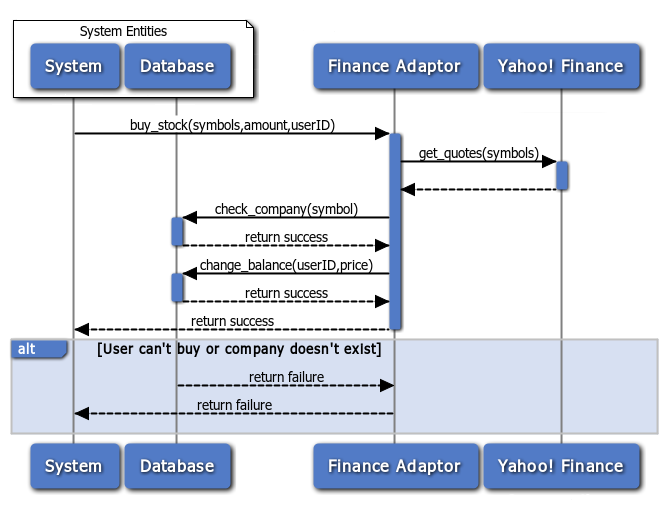
\includegraphics[width=5.5in]{./Diagrams/InteractionDiagrams/buyingstock.png}
\caption{When a user buys a stock, the browser will inform the system of the transaction so that it can be approved. The system passes over the process to the finance adaptor who will check the current price from Yahoo! Finance, check if the company is accepting trades from the database, and check if the user is able to afford the purchase from the database. If all goes well, the transaction will be recorded in the database and the balance will be changed. After all that is complete, the transaction will marked as a success and the system will be notified.}
\end{figure}

\begin{figure}
\centering
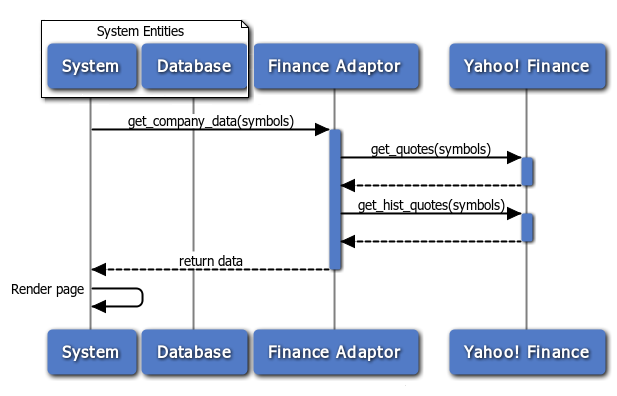
\includegraphics[width=5.5in]{./Diagrams/InteractionDiagrams/rendercompanypage.png}
\caption{When a user wants to view a company page, the company data must be loaded from our finance API. Once the process is passed to the finance adaptor, the quotes and the historical quotes will be pulled from Yahoo! Finance and brought back to the system, who will prepare the page for the user.}
\end{figure}

\begin{figure}
\centering
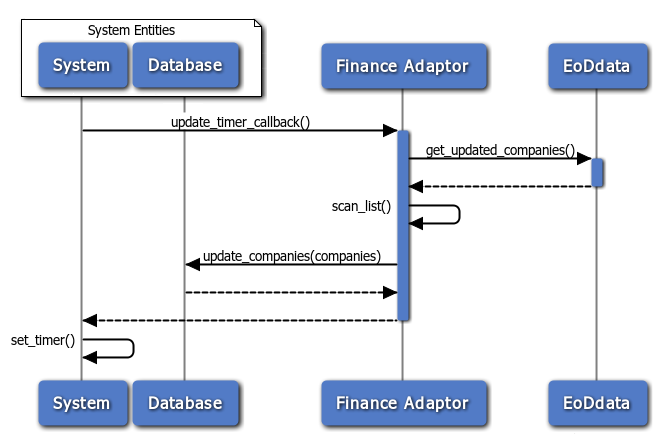
\includegraphics[width=5.5in]{./Diagrams/InteractionDiagrams/updatingdatabase.png}
\caption{We need to keep a local copy of the current companies in our database so we can do rapid processes sing of all of the companies. In order to do this, there will be a timer that is set to update the database every once in a while. When the timer goes off, the system will pass the process onto the finance adaptor. The finance adaptor will then call data from EODData, who knows all of the current companies in the stock market. The finance adaptor will then scan the data for any new/deleted companies and change the database accordingly. After this is complete, the timer will start again so this process can loop.}
\end{figure}
